\documentclass[11pt,a4paper]{article}
\usepackage[utf8]{inputenc}
\usepackage[margin=2cm]{geometry}
\usepackage{graphicx}
\usepackage{amsmath,amssymb}
\usepackage{booktabs}
\usepackage{float}
\usepackage{xcolor}
\usepackage[hidelinks]{hyperref}

\title{\textbf{Valutazione Sperimentale delle Prestazioni degli Algoritmi di Scheduling al Variare del Workload}\texorpdfstring{\\ \large Studio Comparativo su Costellazioni Satellitari LEO (Satellite Edge Computing)}{ - Studio Comparativo su Costellazioni Satellitari LEO (Satellite Edge Computing)}}
\author{\textbf{Claudio Bagini 2045337}}
\date{\today}

\begin{document}

\maketitle

\begin{abstract}
La presente relazione illustra i risultati della campagna sperimentale volta a valutare la scalabilità e la robustezza di nove configurazioni algoritmiche di task offloading al variare sistematico della composizione del carico di lavoro ($\boldsymbol{\beta}$), della dimensione dei dati real-time ($\boldsymbol{\alpha}$), del tasso di arrivo delle richieste ($\lambda \in [2, 10]\text{ req/s}$) e della riserva energetica di bordo ($40\text{ kJ}$ vs $80\text{ kJ}$). 
\end{abstract}

\section{Setup Sperimentale e Parametri di Test}
La campagna ha posto a confronto 9 strategie algoritmiche:
\begin{itemize}
    \item \textbf{Euristiche Decentralizzate:} \texttt{Orbit-aware}, \texttt{DTS-base} e \texttt{DTS-Optimal}.
    \item \textbf{Programmazione Lineare Intera (ILP) Decentralizzata:} \texttt{ILP-Hierarchical (Time)} e \texttt{ILP-Hierarchical (Energy)}.
    \item \textbf{ILP Centralizzato con Batching Dinamico:} valutato nelle varianti con invio rapido ($BS=20, BT=0.05\text{ s}$) e batch convenzionale ($BS=2, BT=2.0\text{ s}$), ciascuna testata con funzione obiettivo mirata alla latenza (\textit{Time}) e al consumo energetico (\textit{Energy}).
\end{itemize}

I parametri di profilazione del carico adottati sono:
\begin{enumerate}
    \item \textbf{Distribuzione delle Tipologie di Task ($\boldsymbol{\beta}$):}
    \begin{itemize}
        \item \textit{Data-Intensive:} $\boldsymbol{\beta} = (0, 0, 1)$ ($100\%$ richieste CPU \& Data-intensive).
        \item \textit{CPU-Intensive:} $\boldsymbol{\beta} = (0, 1, 0)$ ($100\%$ richieste CPU-heavy con payload ridotto).
        \item \textit{Mixed Workload:} $\boldsymbol{\beta} = (0.40, 0.35, 0.25)$ (profilo standard multi-servizio).
    \end{itemize}
    \item \textbf{Distribuzione Dimensionale Real-Time ($\boldsymbol{\alpha}$):} Std $(0.3, 0.5, 0.2)$, L-heavy $(0, 0.7, 0.3)$, VL-heavy $(0, 0.3, 0.7)$ e Pure-L $(0, 1, 0)$.
    \item \textbf{Budget Energetico e Vincoli Temporali:} $E \in \{40, 80\}\text{ kJ}$ e fattore di rilassamento della deadline impostato al $20\%$.
\end{enumerate}


\section{Analisi del Tasso di Successo (Success Rate)}

Il Success Rate misura la frazione di task completati entro la propria deadline e senza violare i budget energetici dei nodi satellite.

\begin{figure}[H]
    \centering
    \makebox[\textwidth][c]{%
        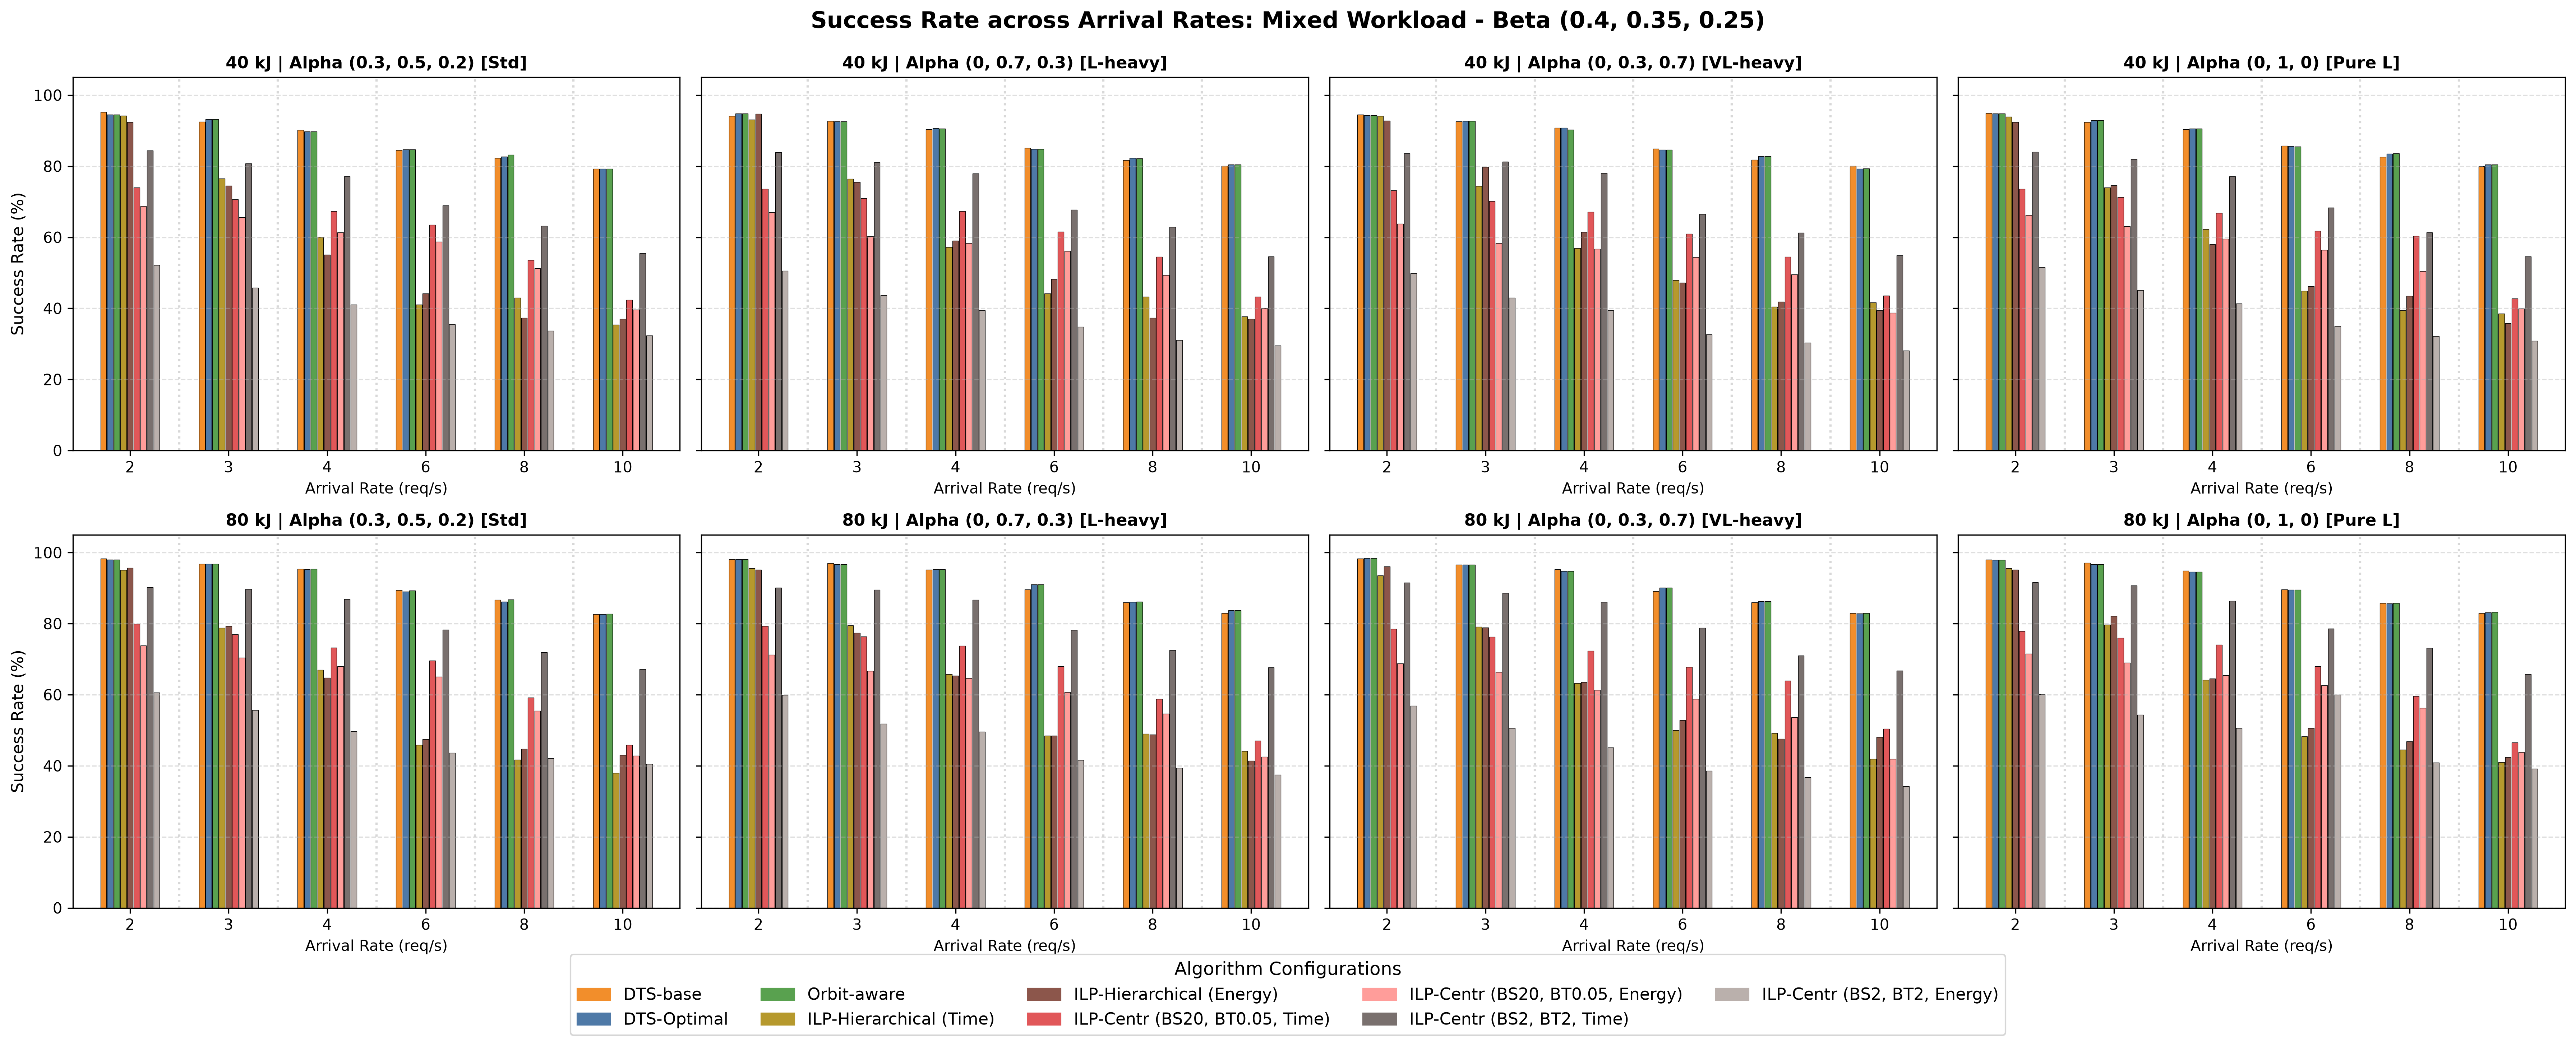
\includegraphics[width=\paperwidth]{01_Success_Rate_Beta___0_4__0_35__0_25.png}%
    }
    \caption{Success Rate per Carico Misto $\boldsymbol{\beta} = (0.40, 0.35, 0.25)$.}
    \label{fig:sr_mixed}
\end{figure}

\begin{figure}[H]
    \centering
    \makebox[\textwidth][c]{%
        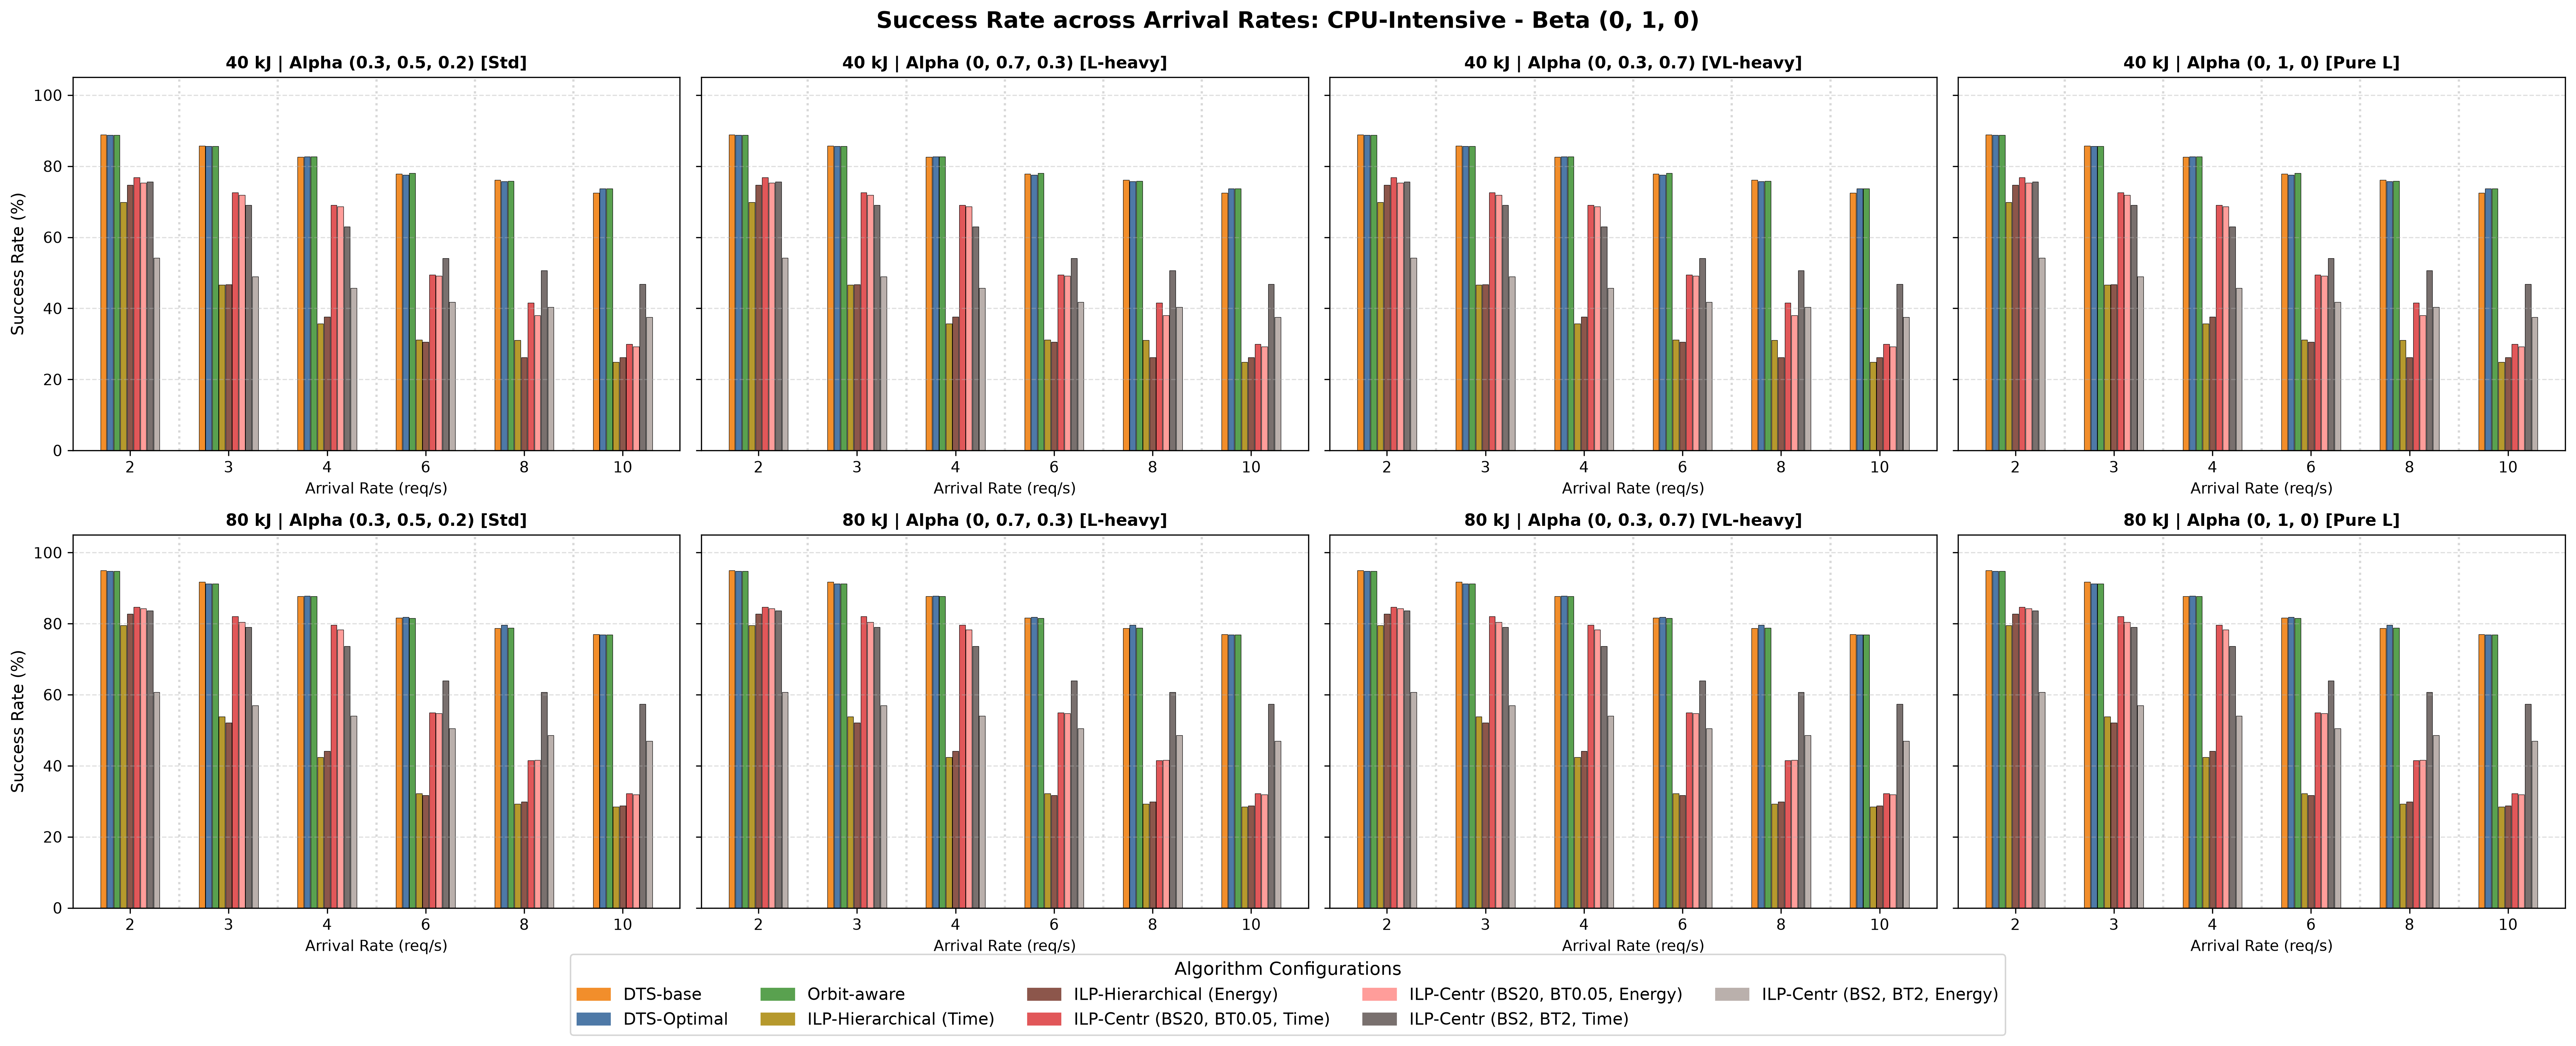
\includegraphics[width=\paperwidth]{01_Success_Rate_Beta___0__1__0.png}%
    }
    \caption{Success Rate per Carico CPU-Intensive $\boldsymbol{\beta} = (0, 1, 0)$.}
    \label{fig:sr_cpu}
\end{figure}

\begin{figure}[H]
    \centering
    \makebox[\textwidth][c]{%
        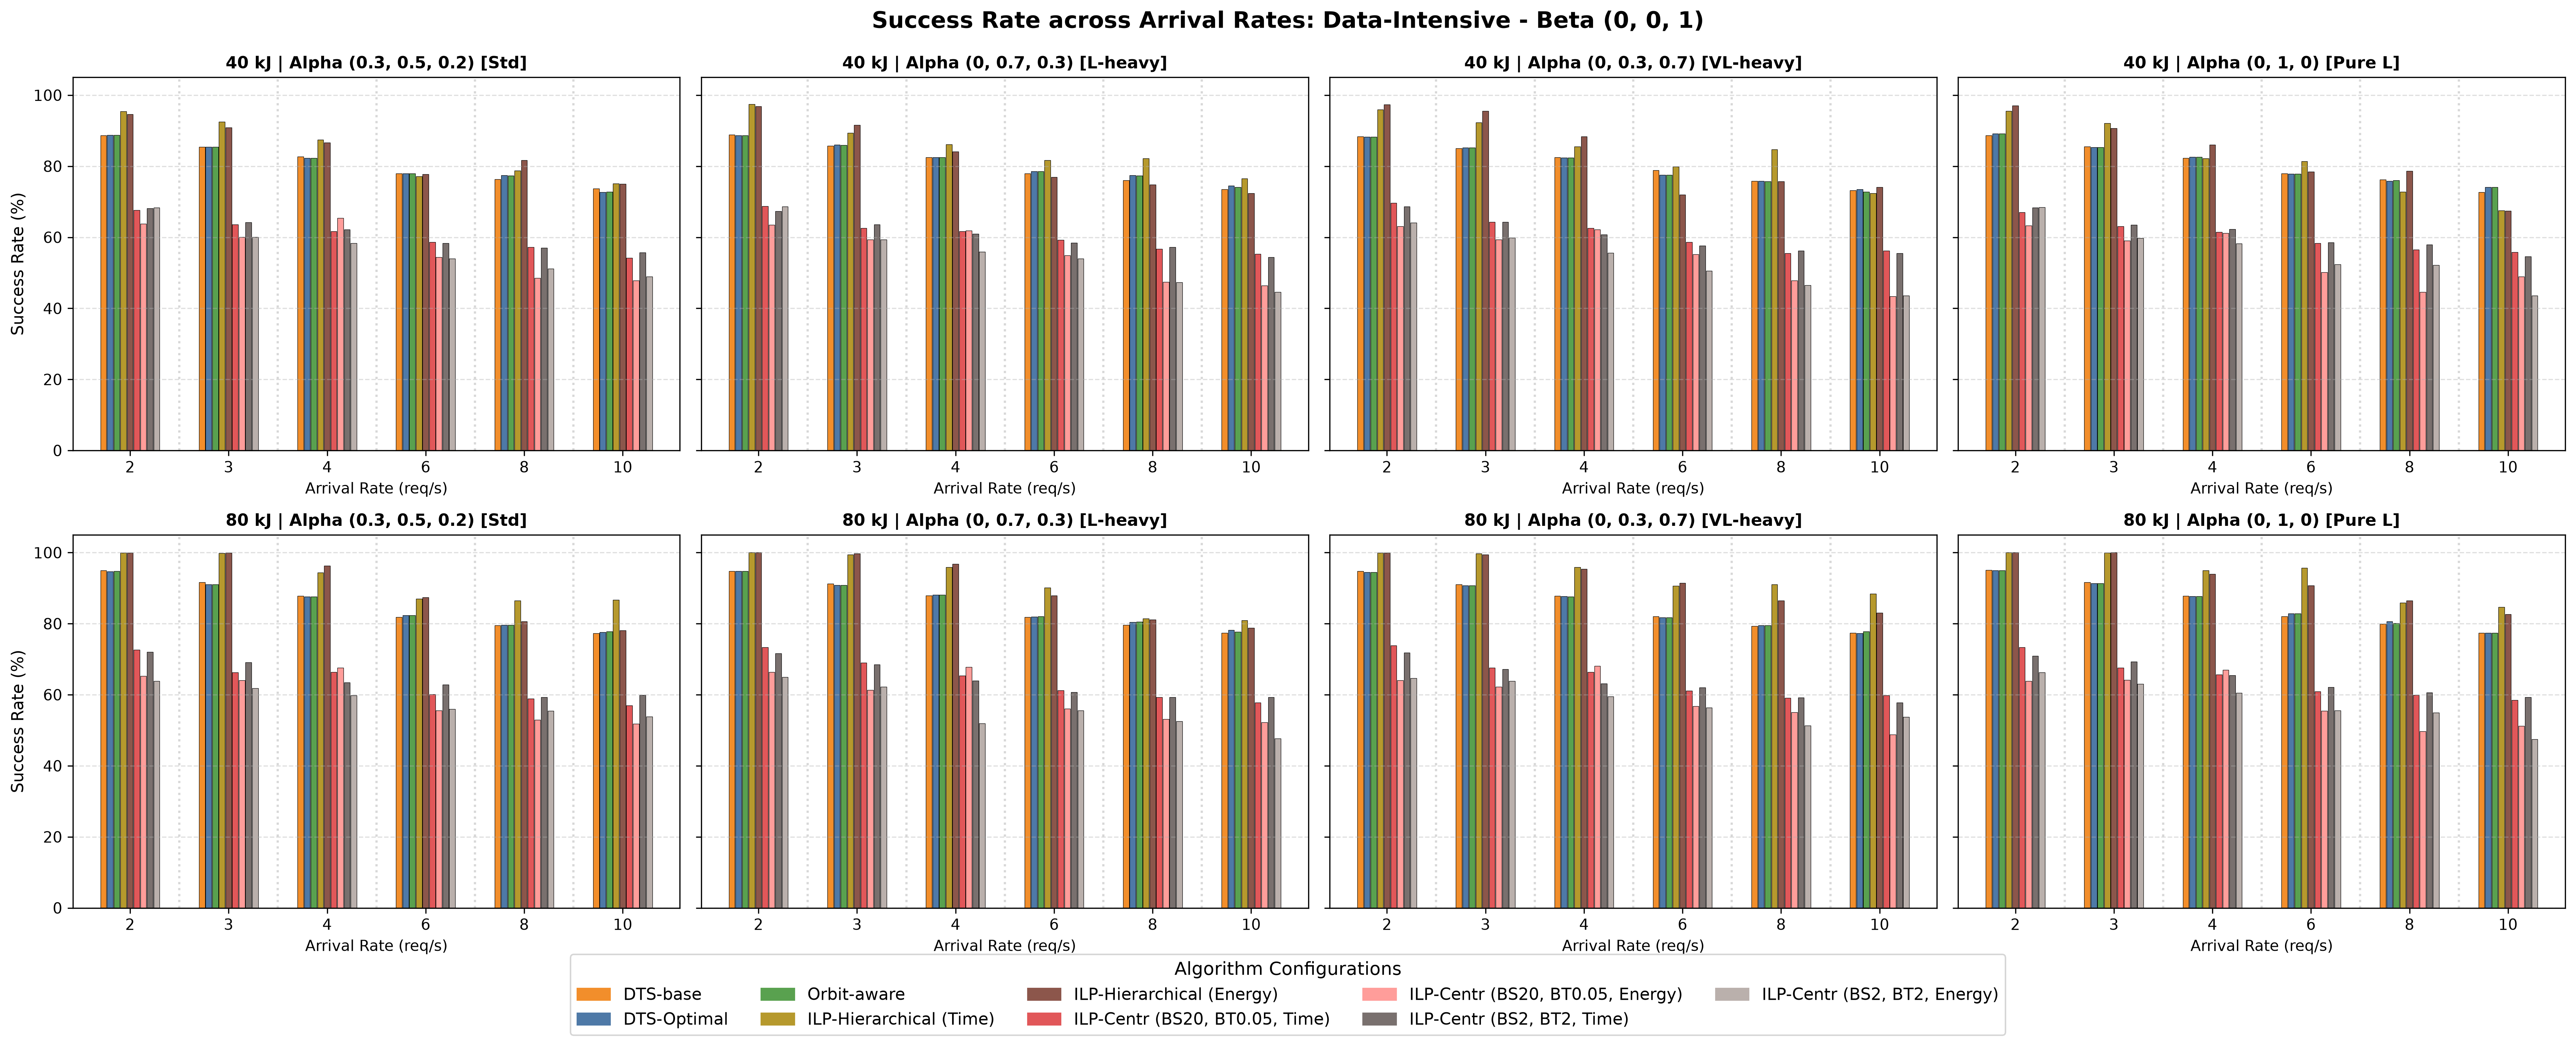
\includegraphics[width=\paperwidth]{01_Success_Rate_Beta___0__0__1.png}%
    }
    \caption{Success Rate per Carico Data-Intensive $\boldsymbol{\beta} = (0, 0, 1)$.}
    \label{fig:sr_data}
\end{figure}

\subsection{Discussione del Success Rate}
\begin{itemize}
    \item \textbf{Resilienza delle Euristiche:} In tutte le configurazioni di $\boldsymbol{\beta}$, gli algoritmi euristici (\texttt{DTS-base}, \texttt{DTS-Optimal}, \texttt{Orbit-aware}) evidenziano un degrado controllato e prevedibile al crescere del tasso di arrivo ($\lambda$). Nel caso misto (Fig.~\ref{fig:sr_mixed}), il tasso di successo scende dal $\sim 95\%$ ($\lambda=2$) a circa l'$80\%$ a massimo stress ($\lambda=10$).
    \item \textbf{Crollo dell'ILP in Scenari CPU-Intensive:} Come visibile in Fig.~\ref{fig:sr_cpu}, l'approccio \texttt{ILP-Hierarchical} collassa drammaticamente all'aumentare di $\lambda$, precipitando a tassi inferiori al $30\%$ già a 8 req/s. In assenza di payload pesanti, la rete non è satura, ma il calcolo simultaneo di allocazioni matematicamente complesse induce ritardi insostenibili.
    \item \textbf{Efficacia dell'ILP in Ambito Data-Intensive:} In Fig.~\ref{fig:sr_data}, \texttt{ILP-Hierarchical (Time)} raggiunge prestazioni di picco a basso traffico ($98\text{--}100\%$ a 2 req/s) e beneficia in modo marcato dell'estensione del budget a $80\text{ kJ}$, mantenendosi sopra l'$80\%$ anche a $\lambda=10$. In presenza di trasferimenti ingenti, l'ottimizzazione globale dei percorsi ISL ripaga il costo computazionale.
    \item \textbf{Ruolo del Batch Timeout ($BT$):} L'ILP centralizzato con $BT=0.05\text{ s}$ domina stabilmente la variante con $BT=2.0\text{ s}$, dimostrando che attendere l'accumulo di un batch ampio è deleterio per i vincoli di deadline.
\end{itemize}


\section{Diagnostica delle Cause di Scarto (Rejection Causes)}

L'analisi della distribuzione delle cause di fallimento rivela l'origine intrinseca del collasso prestazionale.

\begin{figure}[H]
    \centering
    \makebox[\textwidth][c]{%
        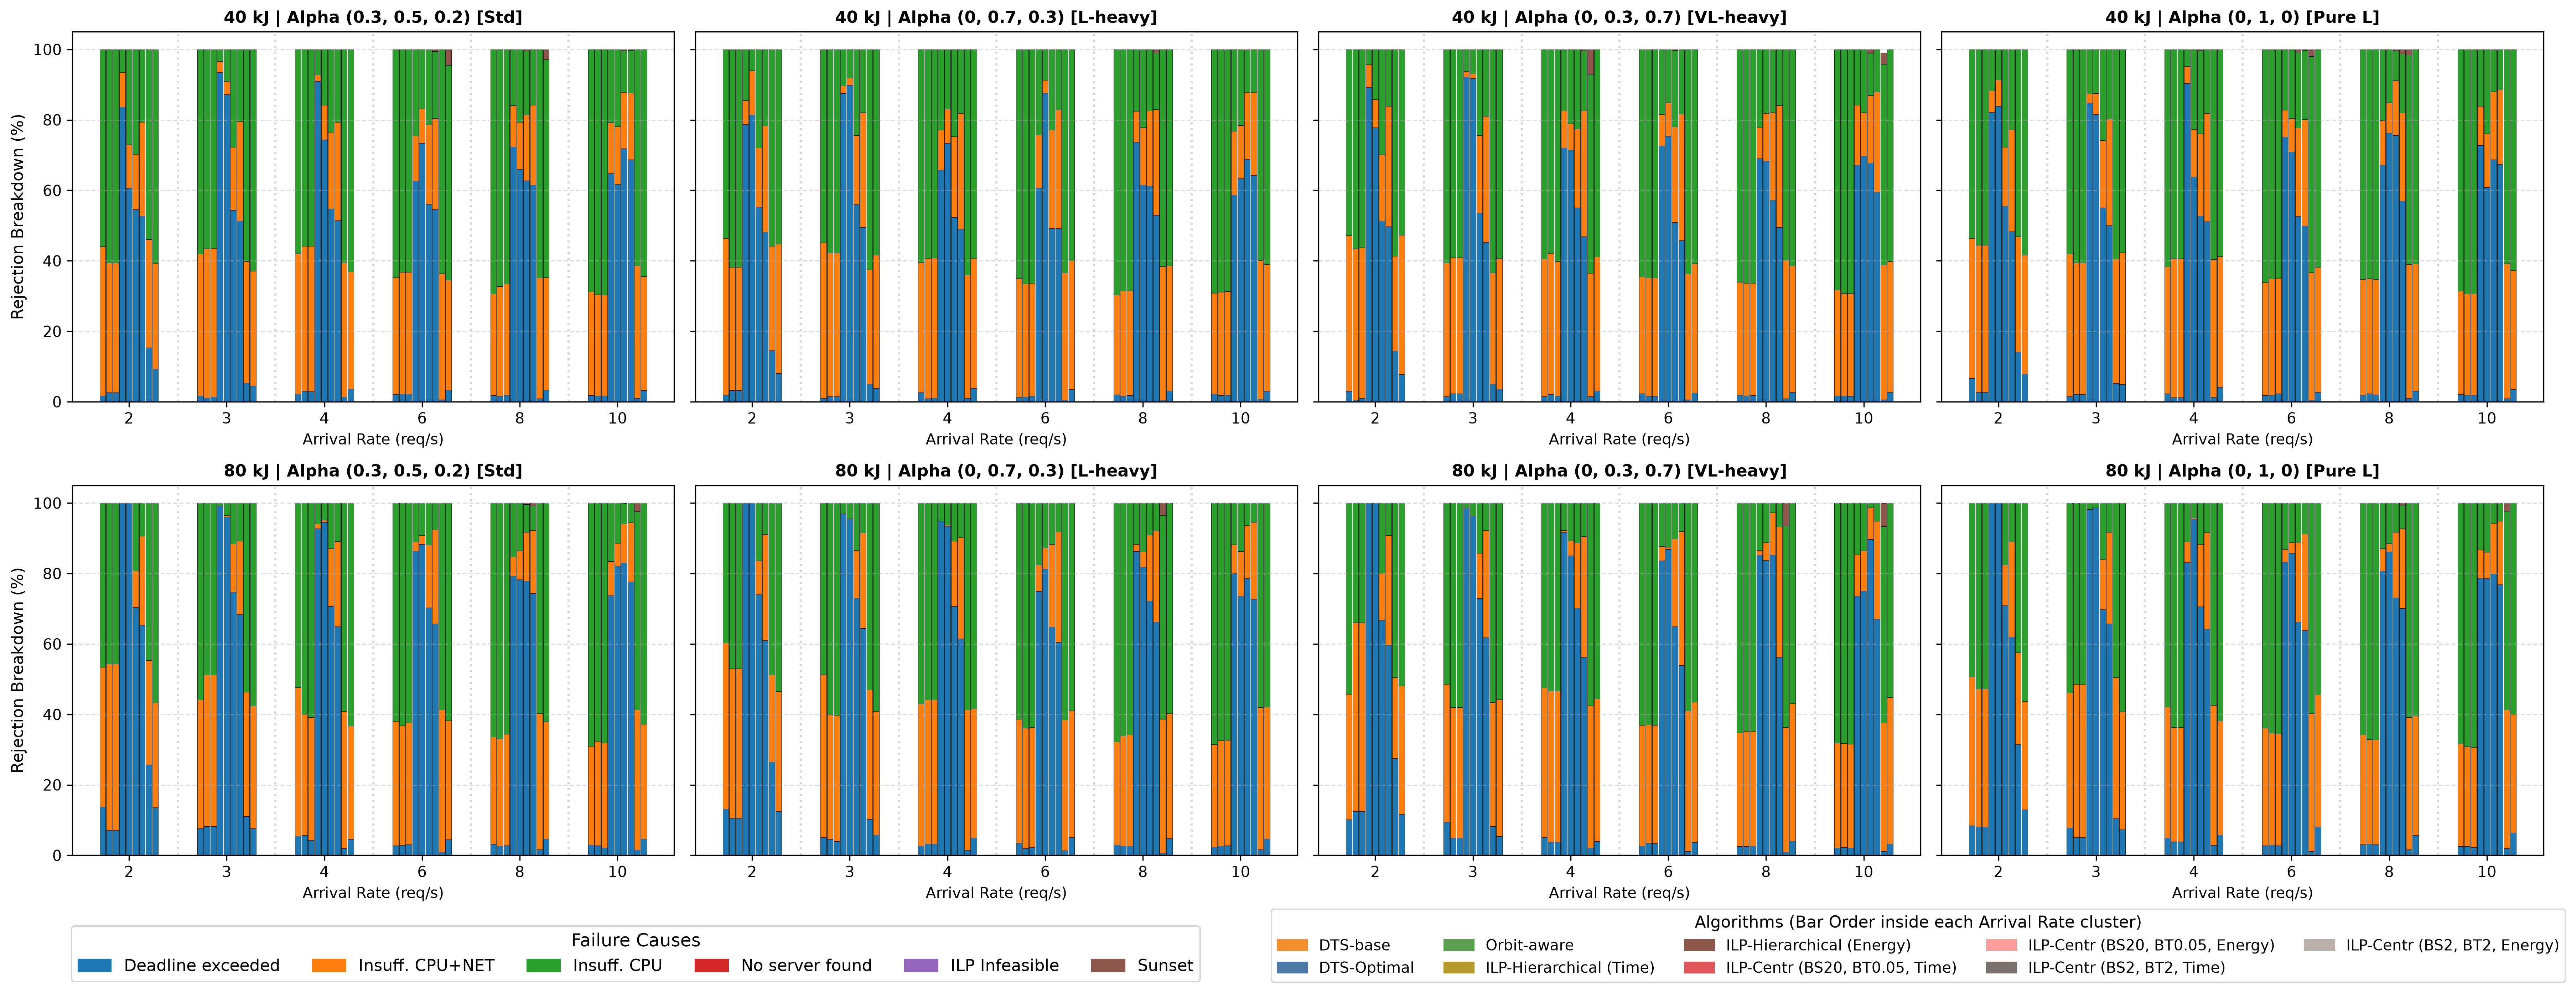
\includegraphics[width=\paperwidth]{03_Rejection_Causes_Beta___0_4__0_35__0_25.png}%
    }
    \caption{Distribuzione cause di rigetto per Carico Misto $\boldsymbol{\beta} = (0.40, 0.35, 0.25)$.}
    \label{fig:rej_mixed}
\end{figure}

\begin{figure}[H]
    \centering
    \makebox[\textwidth][c]{%
        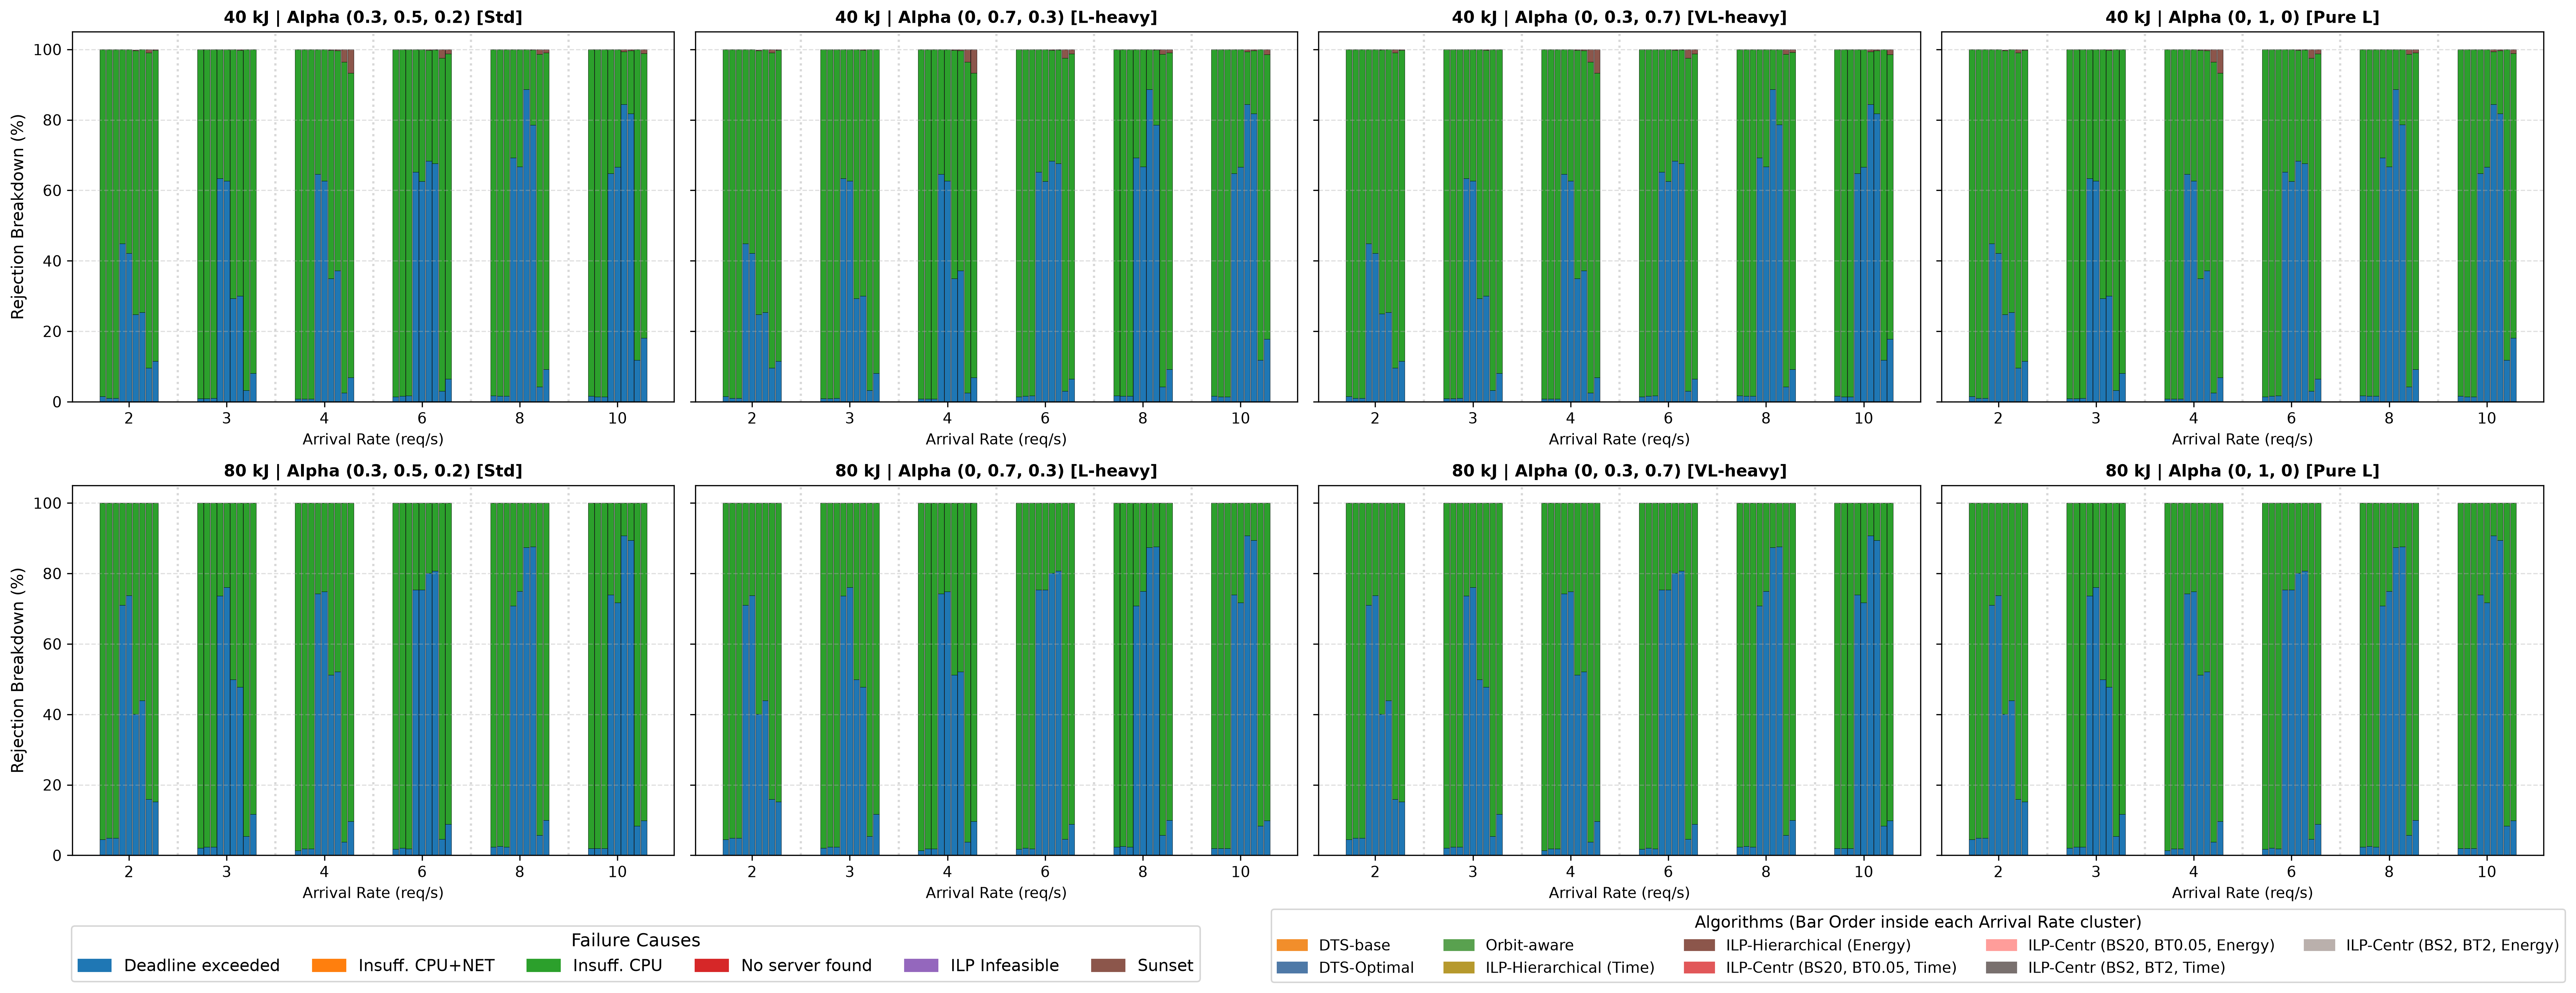
\includegraphics[width=\paperwidth]{03_Rejection_Causes_Beta___0__1__0.png}%
    }
    \caption{Distribuzione cause di rigetto per Carico CPU-Intensive $\boldsymbol{\beta} = (0, 1, 0)$.}
    \label{fig:rej_cpu}
\end{figure}

\begin{figure}[H]
    \centering
    \makebox[\textwidth][c]{%
        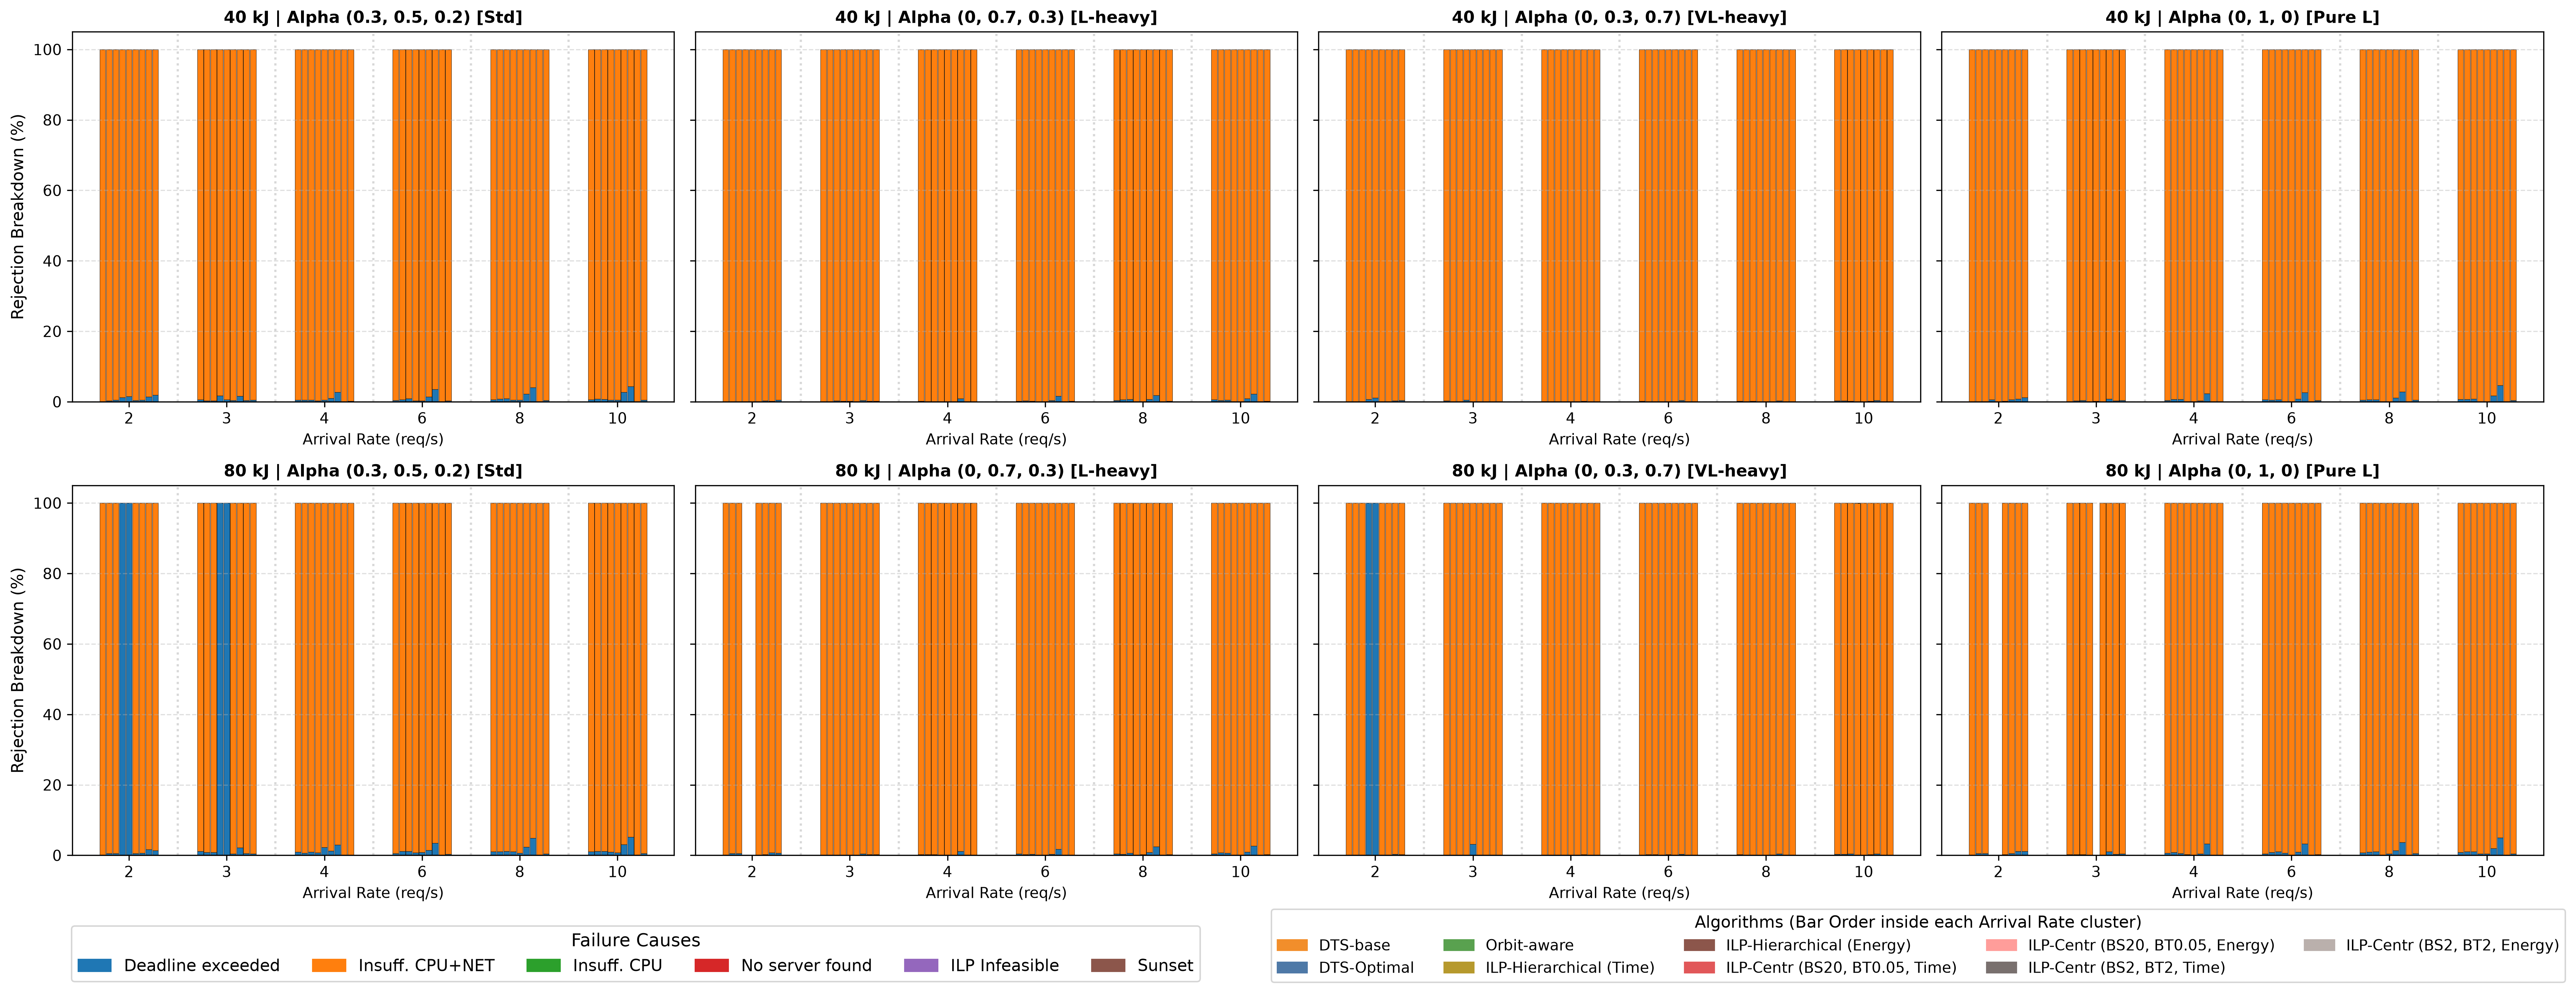
\includegraphics[width=\paperwidth]{03_Rejection_Causes_Beta___0__0__1.png}%
    }
    \caption{Distribuzione cause di rigetto per Carico Data-Intensive $\boldsymbol{\beta} = (0, 0, 1)$.}
    \label{fig:rej_data}
\end{figure}

\subsection{Discussione delle Cause di Scarto}
\begin{itemize}
    \item \textbf{Data-Intensive (Fig.~\ref{fig:rej_data}):} Per tutti gli algoritmi analizzati, oltre il $95\%$ dei fallimenti è contrassegnato da \textbf{\texttt{Insuff. CPU+NET}} (arancione). Il fattore limitante primario non è la scadenza temporale, bensì l'esaurimento della capacità di trasmissione sui link ISL e dell'energia spesa per la movimentazione dei file di grandi dimensioni ($20\text{--}50\text{ MB}$).
    \item \textbf{Dicotomia Netta nel CPU-Intensive (Fig.~\ref{fig:rej_cpu}):} Si osserva una netta contrapposizione sistemica:
    \begin{enumerate}
        \item Le \textbf{euristiche} rigettano i task al $100\%$ per \textbf{\texttt{Insuff. CPU}} (verde). La decisione di inoltro è istantanea; il task non accumula ritardo artificiale e viene respinto solo se la coda di esecuzione computazionale del target è fisicamente piena.
        \item I modelli \textbf{ILP} (sia gerarchici che centralizzati) vedono la quota di \textbf{\texttt{Deadline exceeded}} (blu) salire dal $40\%$ fino all'$85\text{--}90\%$ a pieno carico ($\lambda=10$). Questo comprova inequivocabilmente che i task non falliscono per indisponibilità hardware, ma per l'eccessivo tempo di residenza nel sistema durante l'elaborazione del piano di scheduling.
    \end{enumerate}
    \item \textbf{Carico Misto (Fig.~\ref{fig:rej_mixed}):} Presenta una composizione mista in cui le euristiche ripartiscono gli scarti tra saturazione CPU e CPU+NET, confermando l'assenza di scarti per scadenza deadline.
\end{itemize}


\section{Scomposizione dei Tempi di Risposta (Response Time)}

Il tempo di risposta totale è disaggregato in tempo di esecuzione sui nodi (\textit{System Execution}) e latenza di attesa/trasmissione di rete (\textit{Network / Wait Time}).

\begin{figure}[H]
    \centering
    \makebox[\textwidth][c]{%
        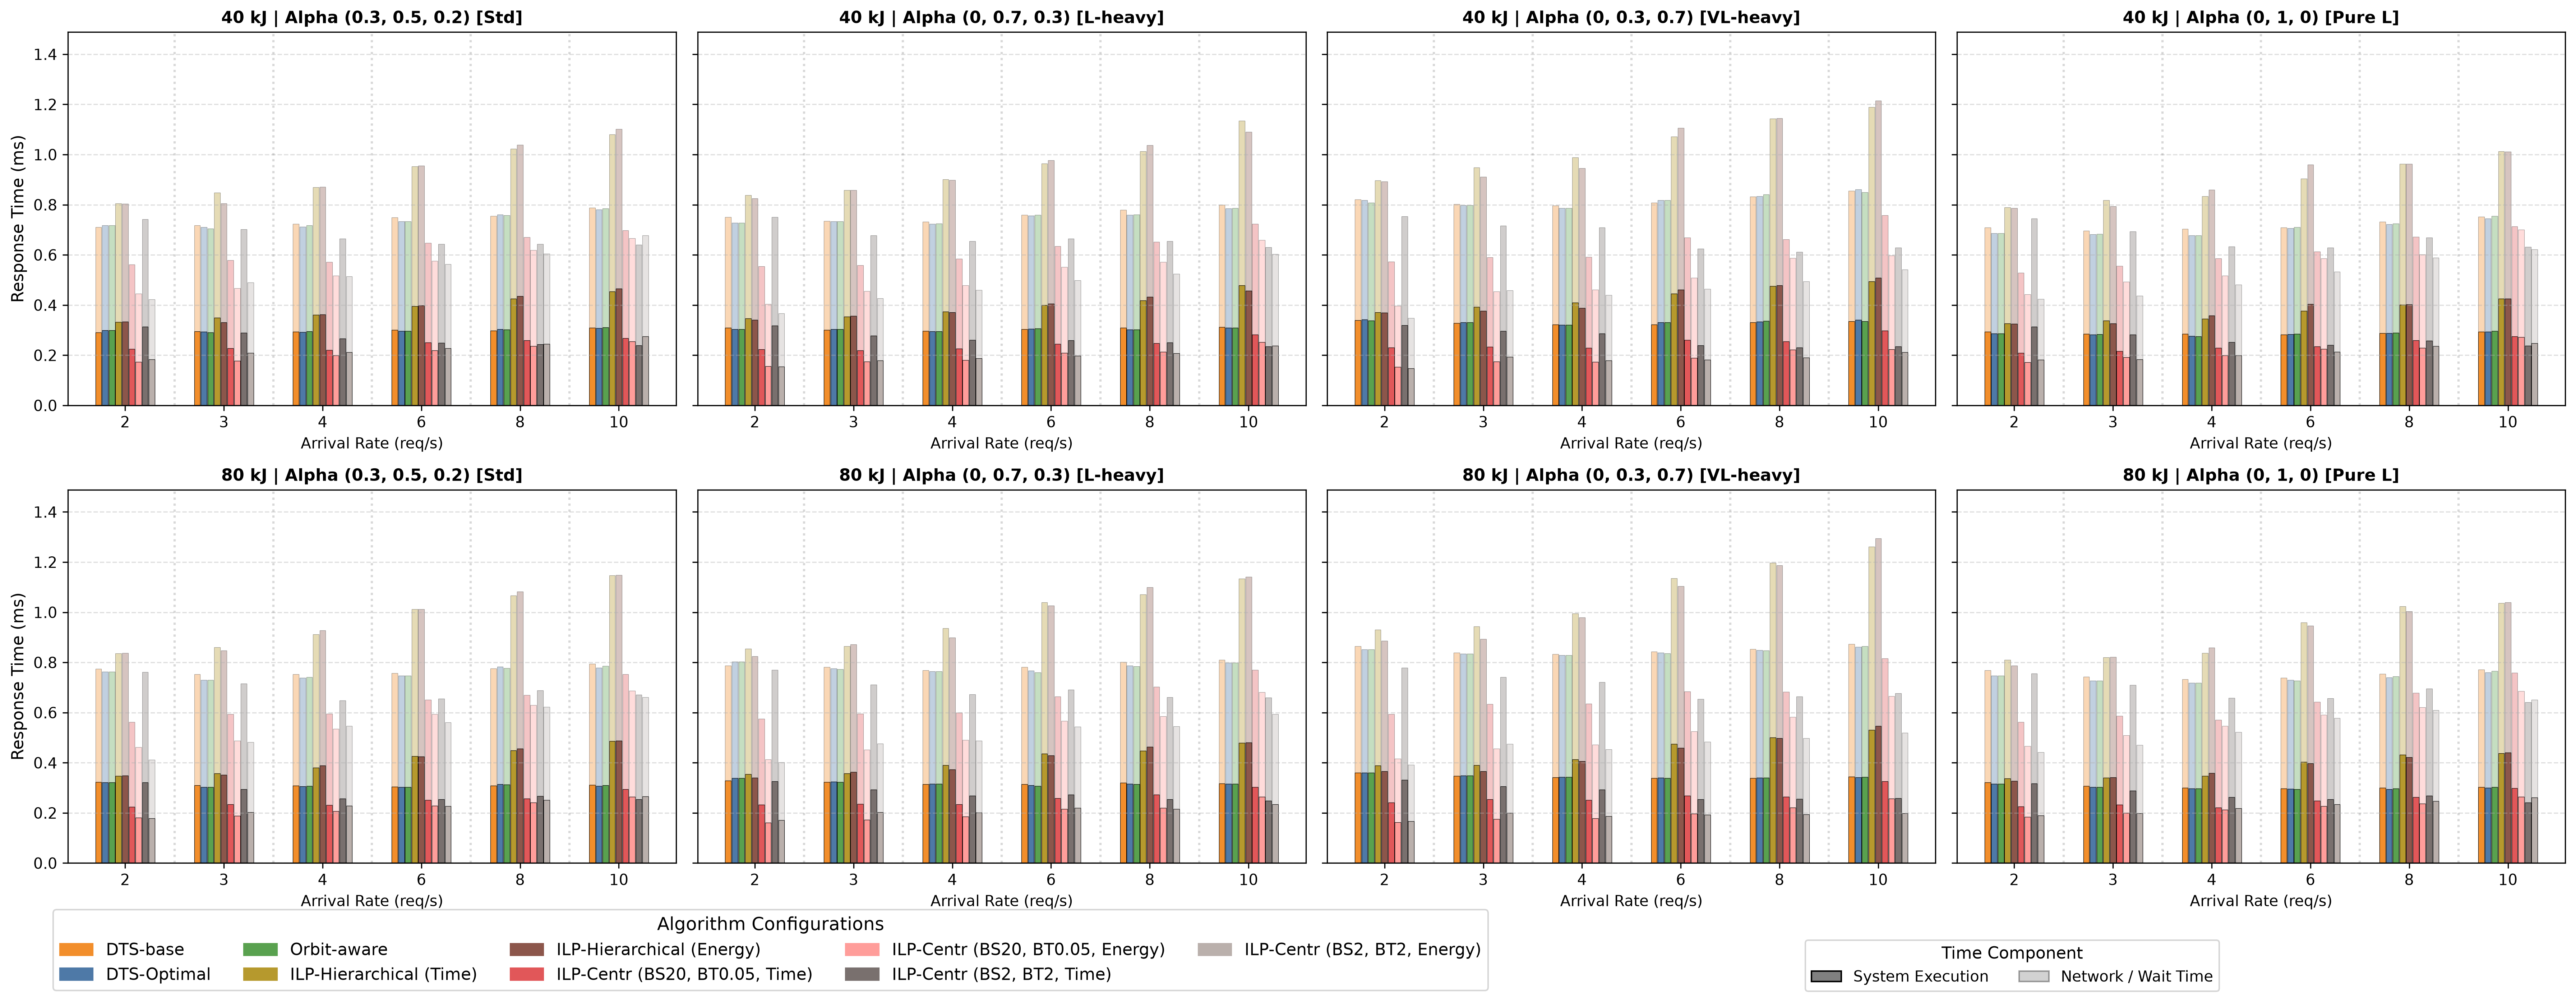
\includegraphics[width=\paperwidth]{02_Response_Time_Beta___0_4__0_35__0_25.png}%
    }
    \caption{Response Time stacked per Carico Misto $\boldsymbol{\beta} = (0.40, 0.35, 0.25)$.}
    \label{fig:rt_mixed}
\end{figure}

\begin{figure}[H]
    \centering
    \makebox[\textwidth][c]{%
        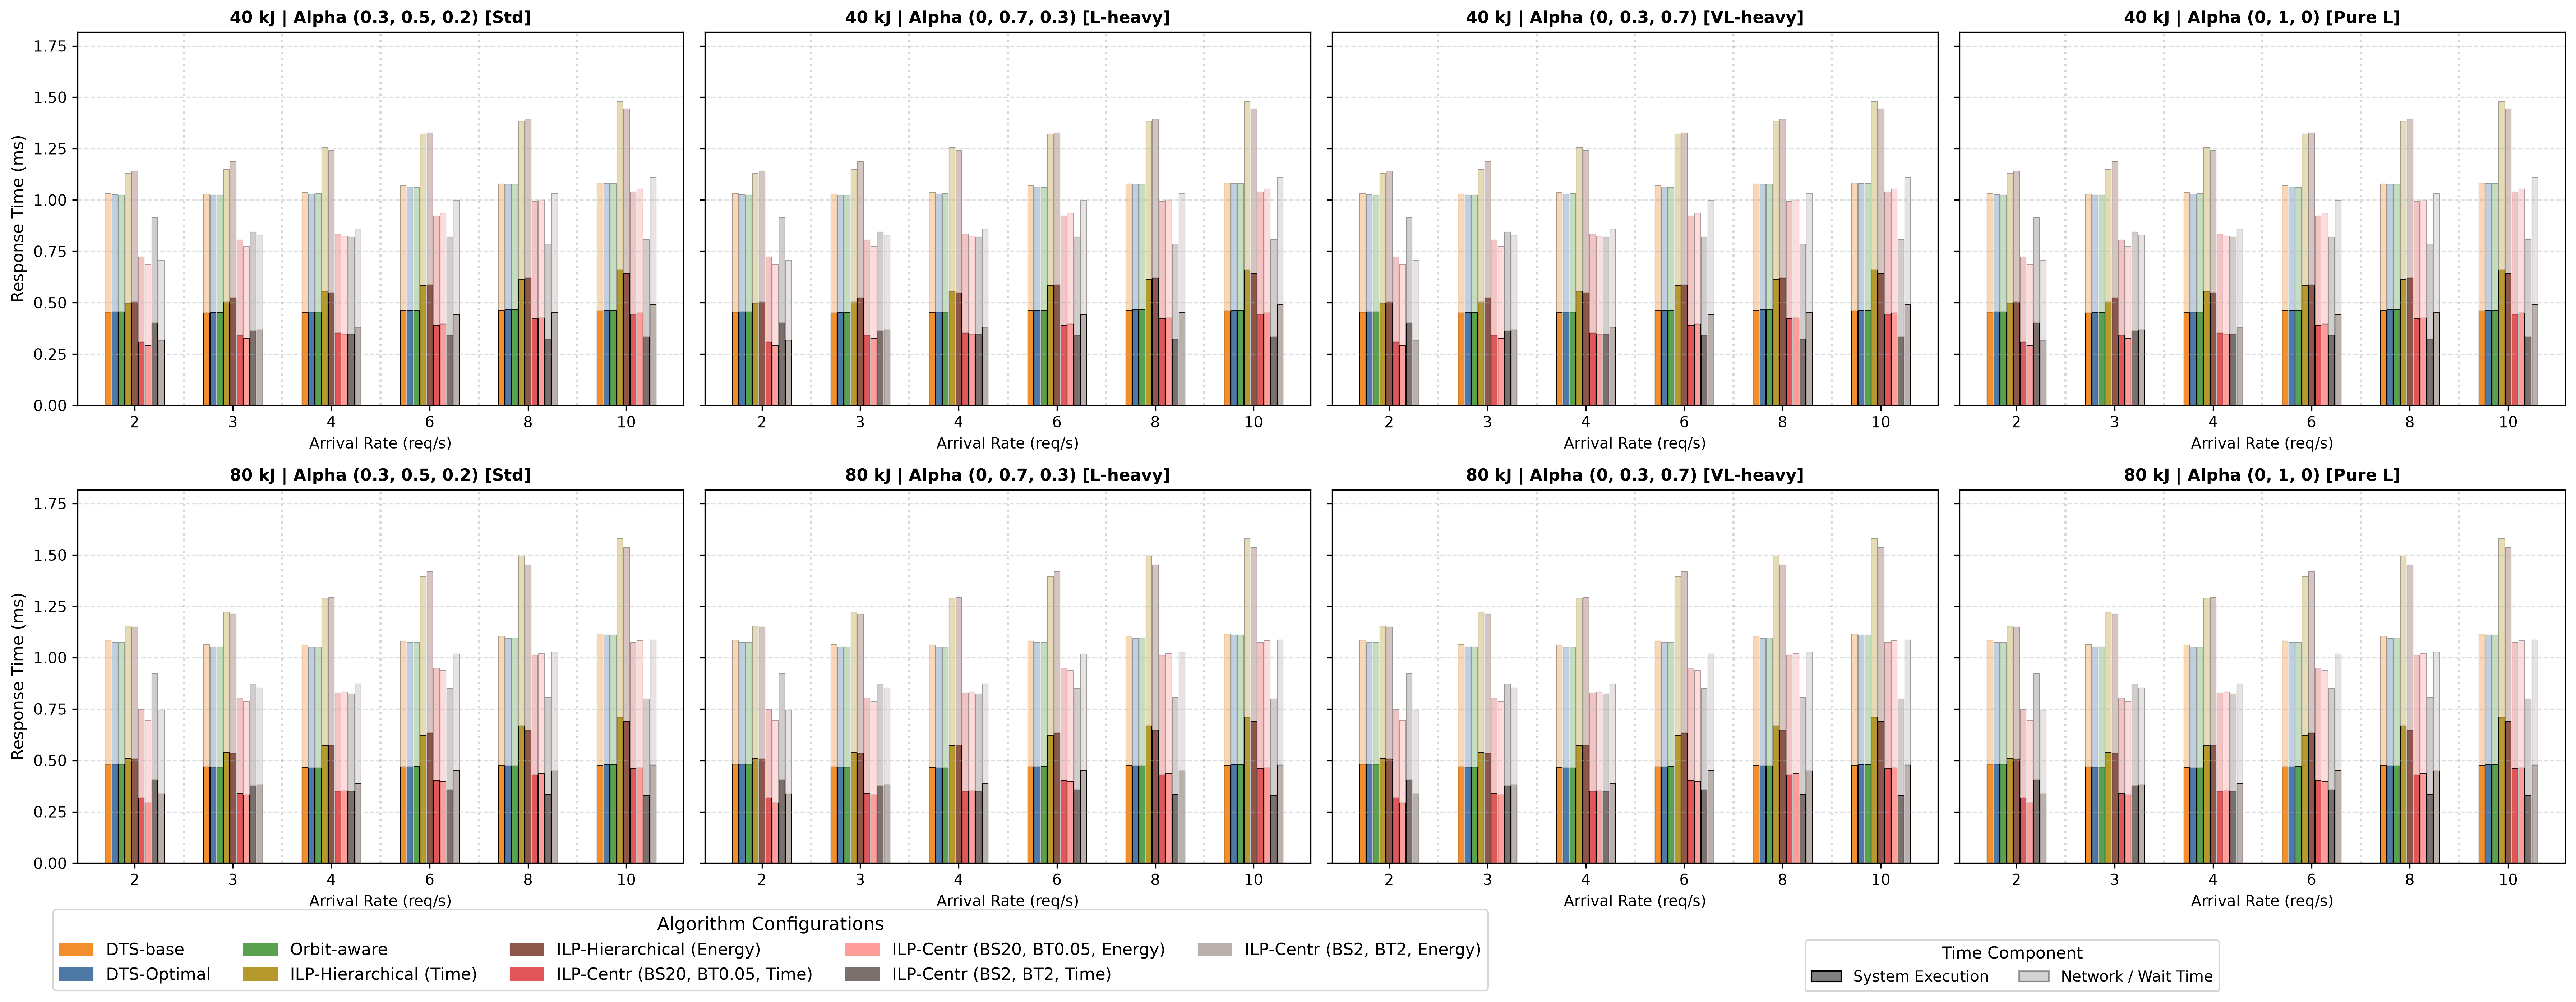
\includegraphics[width=\paperwidth]{02_Response_Time_Beta___0__1__0.png}%
    }
    \caption{Response Time stacked per Carico CPU-Intensive $\boldsymbol{\beta} = (0, 1, 0)$.}
    \label{fig:rt_cpu}
\end{figure}

\begin{figure}[H]
    \centering
    \makebox[\textwidth][c]{%
        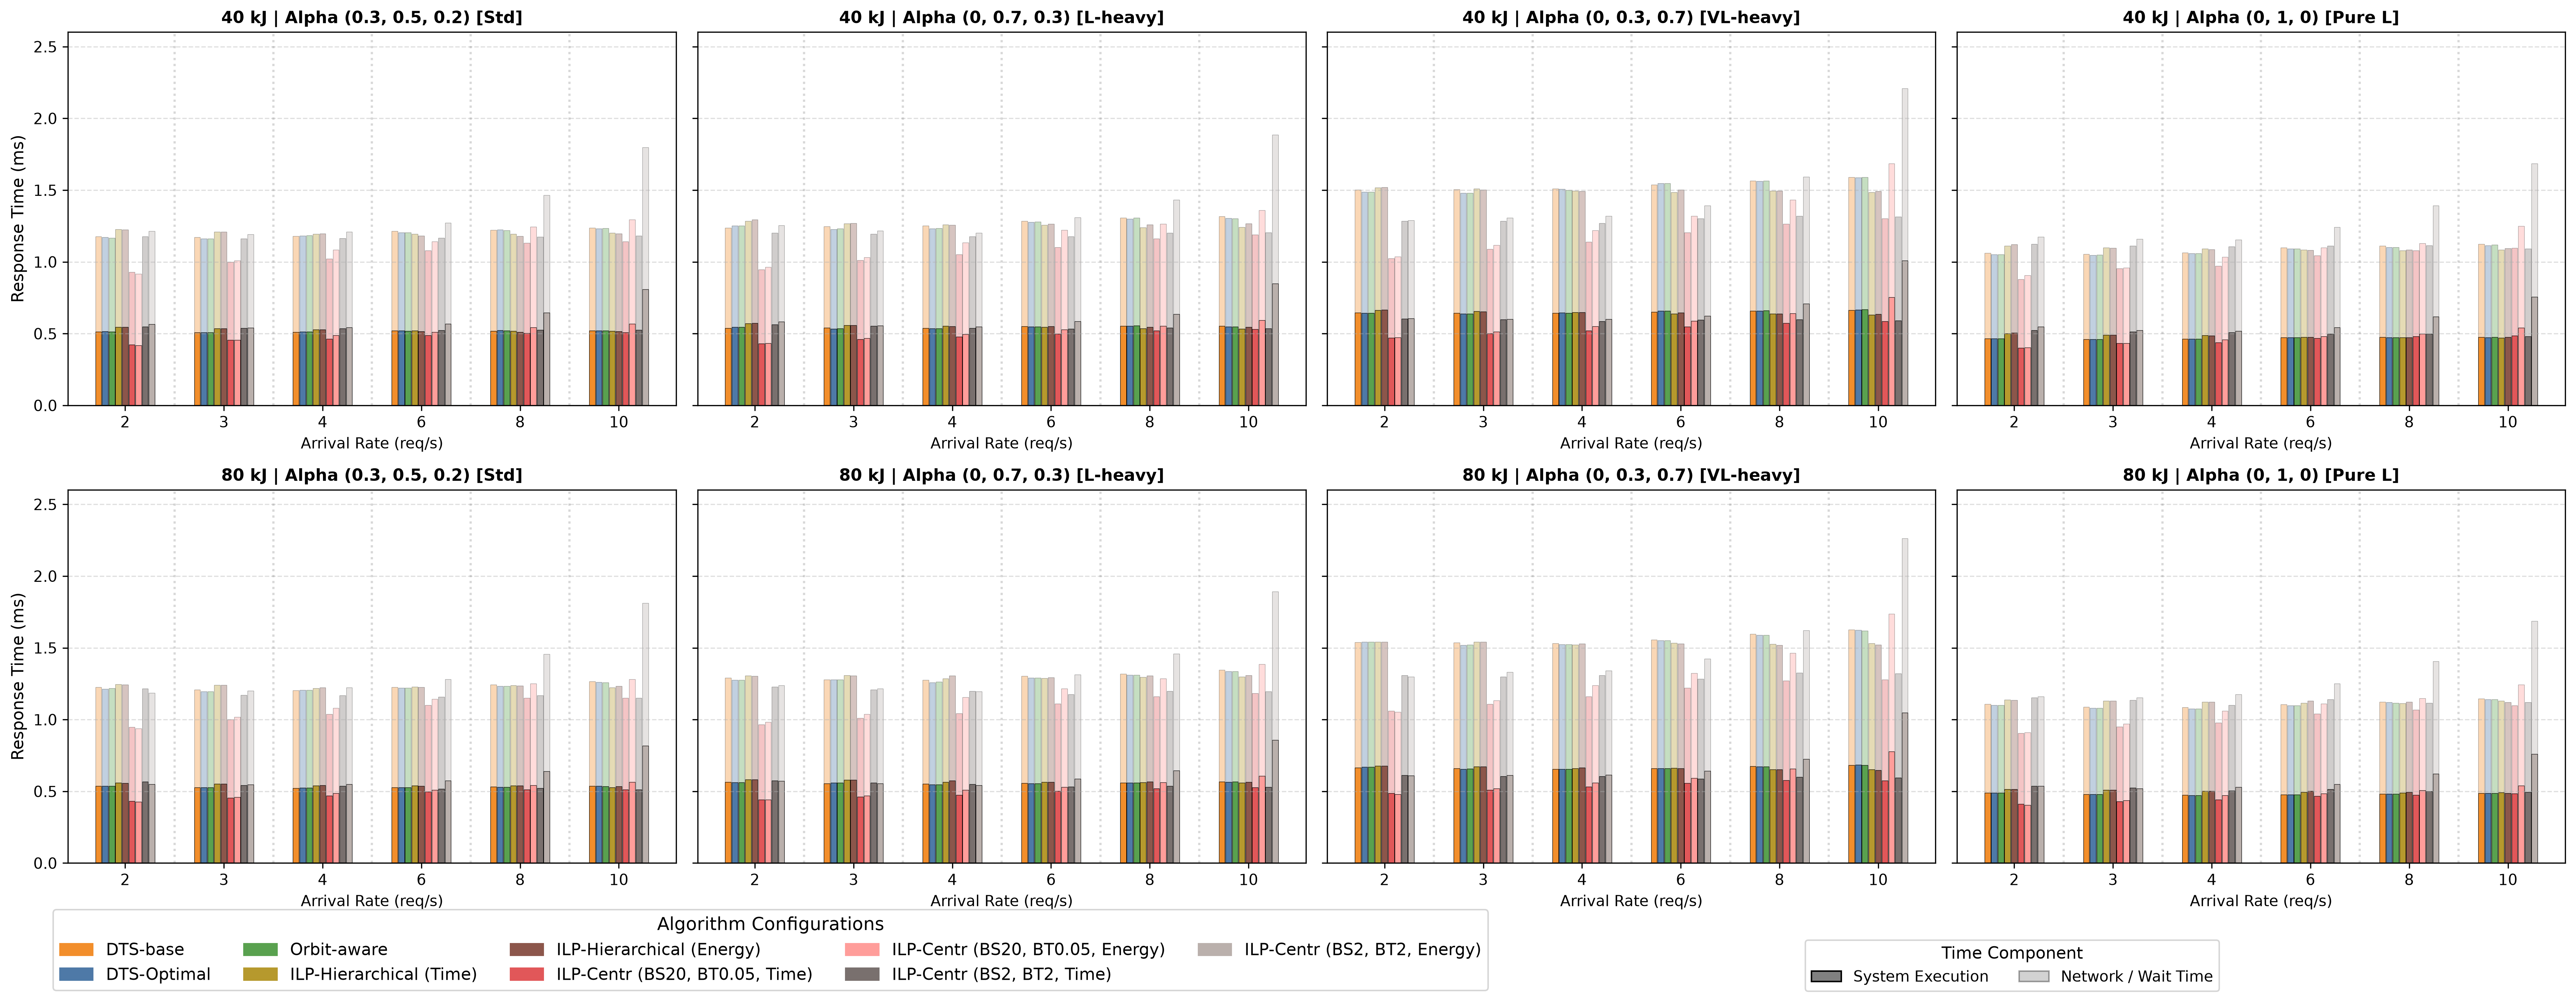
\includegraphics[width=\paperwidth]{02_Response_Time_Beta___0__0__1.png}%
    }
    \caption{Response Time stacked per Carico Data-Intensive $\boldsymbol{\beta} = (0, 0, 1)$.}
    \label{fig:rt_data}
\end{figure}

\subsection{Discussione sui Tempi di Risposta}
\begin{itemize}
    \item \textbf{Stabilità delle Euristiche:} \texttt{Orbit-aware} e le varianti \texttt{DTS} evidenziano una latenza orizzontale praticamente costante ($0.7\text{--}1.1\text{ ms}$), con tempi di esecuzione stabili indipendentemente dal tasso di arrivo delle richieste.
    \item \textbf{Impatto del Batch Timeout sul Centralizzato:} La configurazione \texttt{ILP-Centr (BS20, BT0.05)} registra latenze minime ($\approx 0.6\text{--}0.7\text{ ms}$), paragonabili o inferiori alle euristiche a basso carico. Al contrario, l'adozione di un timeout conservativo ($BT=2.0\text{ s}$) causa un'esplosione della componente di attesa in coda (\textit{Wait Time}), portando la latenza verso $1.8\text{--}2.0\text{ ms}$.
\end{itemize}
\end{document}